% !TeX root = ..//diffgeo_main.tex

Im Folgenden ist $\mfk$ immer eine Zusammenhängende Riemansche Mannigfaltigkeit.

\begin{defs}[Geodätisch Vollständig]
    Sei $p \in \mfk$, dann heißt $\mfk$ geodätisch vollständig in $p$, 
    falls $\exp_p$ auf ganz $T_p \mfk$ definiert ist,
    das heißt alle Geodätischen durch $p$ auf ganz $\R$ definiert sind.
\end{defs}

\begin{bsp}
    \label{bsp:geodvollstaendig}
    \begin{enumerate}
        \item $(\R^n, g_{\text{Eukl}})$ ist geodätisch vollständig
        \item $B_1 (0) = \{ x \in \R^n \vert \norm{x} < 1 \}$ ist nicht geodätisch vollständig
    \end{enumerate}
\end{bsp}



\section{Satz von Hopf-Rinow}

\begin{satz}[von Hopf-Rinow]
    \label{satz:hopfrinow}   
    Sei $\mfk$ wie oben eine Zusammenhängende Riemannsche Mannigfaltigkeit. 
    Ferner sei $p \in \mfk$, dann sind folgende Aussagen äquivalent:
    \begin{itemize}
    \item[i)] $\mfk$ ist geodätisch vollständig im Punkt $p$
    \item[ii)] $\mfk$ ist geodätisch vollständig in allen Punkten $q \in \mfk$
    \item[iii)] $\overline{B}_r (p)$ sind kompakt für alle $r > 0, r \in \R$
    \item[iv)] $B_r (q)$  sind kompakt für alle $r \in \R_+$ und alle $ q \in \mfk$
    \item[v)] $(\mfk, d)$ ist ein vollständiger metrischer Raum, 
    d.h. alle Cauchy-Folgen konvergieren
    \end{itemize}
    Jeder der Bedingungen $i)$ - $v)$ impliziert die folgende Aussage:
    \begin{itemize}
    \item[vi)] Jeder Punkt $q \in \mfk$ lässt sich mit $p$ durch eine 
    minimale Geodätische verbinden.
    \end{itemize}
\end{satz}

\begin{bem}
Aussage $vi)$ ist schwächer als die Aussage $i)$ - $v)$ 
(Vergleich: Beispiel \ref{bsp:geodvollstaendig}) 
\end{bem}


\begin{defs}[Vollständige Riemannsche Mannigfaltigkeit]
    Eine Riemannsche Mannigfaltigkeit $\mfk$, die  $i)$ - $v)$ erfüllt, 
    heißt vollständige Riemannsche Mannigfaltigkeit.
\end{defs}

\begin{kor}
    \label{kor:kompaktvoll}
    Jede kompakte Mannigfaltigkeit ist vollständig.
\end{kor}
\begin{bew}[Korollar \ref{kor:kompaktvoll}]
Es genügt $iii)$ von Satz \ref{satz:hopfrinow} zu zeigen.\\
$\overline{B}_r(p) \subset \mfk$ abgeschlossen und da $\mfk$ kompakt folgt, 
dass $\overline{B}_r (p)$ kompakt ist.    
\end{bew}

\begin{bew}[Satz von Hopf-Rinow \ref{satz:hopfrinow}]
    Die Beweisstruktur ist in der Abbildung \ref{fig:proofhopfrinow} zu sehen
    \begin{figure}[H]
        \centering
        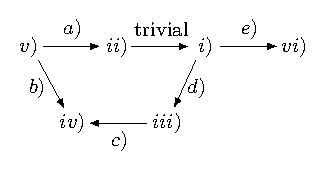
\includegraphics[width=0.5\linewidth]{figures/tikz/proofhopfrinow.pdf}
        \caption{Beweisstruktur für den Satz von Hopf-Rinow}
        \label{fig:proofhopfrinow}
    \end{figure} 


\textbf{zu a):}\\
Sei $c : (\alpha , \beta) \to \mfk$ eine Geodätische mit maximalen Definitionsbereich.
O.B.d.A nehmen wir an, dass $c$ nach der Bogenlänge parametrisiert ist. 
Wir wollen Beweis per Widerspruch führen, das heißt wir nehmen an, 
dass $\beta < \infty$ (Der Fall $\alpha > - \infty$ wir analog durchgeführt).
Dann gilt für eine Folge $t_i \in (\alpha , \beta)$ mit $t_i \to \beta$ für $i \to \infty$.
\begin{align*}
    \dd (c (t_i), c(t_j)) \leq L (c \eval_{[t_i , t_j ]}) = \abs{t_i - t_j}
\end{align*}
Folglich ist $(c(t_i))_{i \in \mathbb{N}}$ eine Cauchy-Folge in $(\mfk , \dd)$. 
Da $(\mfk, \dd)$ vollständig ist folgt, 
dass $q \in \mfk$ existieren mit $c(t_i) \overset{i \to \infty}{\longrightarrow}q$.\\
\textbf{Behauptung:}\\
$q$ hängt nicht von der Wahl der Folge $t_i$ ab.

\begin{bew}[Behauptung]
Sei $(\tilde{t}_i)_{i \in \mathbb{N}}$ eine zweite solche Folge mit 
$\tilde{q} = \lim_{i\to\infty} c(\tilde{t}_i)$ dann definieren wir:
\begin{align}
    \hat{t}_i = \left\{
\begin{array}{ll}
t_j & i = 2 j \\
\tilde{t}_j & i = 2j + 1 \\
\end{array}
\right.
\end{align}
Die Folge $c(\hat{t}_i)$ ist eine Cauchy Folge mit Häufungspunkten $q$ und $\tilde{q}$.
\end{bew}
\textbf{Fortsetzung Beweis}\\

Mit anderen Worten: wir erhalten eine stetige Fortsetzung
$\bar{c}: (\alpha , \beta ] \to \mfk$ von $c$ durch

\begin{align*}
    \bar{c}(t) = \left\{
\begin{array}{ll}
c(t) & \, t\in (\alpha , \beta ) \\
q & \, t = \beta \\
\end{array}
\right.
\end{align*}

\textbf{Behauptung:}\\
$\dot{c}$ besitzt eine stetige Fortsetzung auf $( \alpha , \beta ]$.

\begin{bew}[Behauptung]
Sei $x : U \to V$ eine Karte von $\mfk$ um $q$ mit $x(q)=0$.
Ferner wähle $r > 0$ so, dass $\overline{B}_r (0) \subset V$.
Da $\overline{B}(0)$ kompakt ist, existieren Konstanten $c_1, c_2, c_3 > 0$ so, dass
\begin{enumerate}
\item $\abs{\Gamma^k_{ij}} \leq c_1$, $\forall y \in \overline{B}_r (0)$
\item $\norm{a}_{\text{max}} \leq c_2 \norm{\sum_j a^j \pdv{x_j}\eval{x^{-1}(y)}}_g$
    für alle $a \in \R^n$ und $y \in \overline{B}_r (0)$
\item $\abs{\pdv{\Gamma^k_{ij} (y)}{x_i}} \leq c_3$ für alle $y \in \overline{B}_r (0)$
\end{enumerate}

Setze $c_k = x_k \circ c$ und $a_k = \dot{c}_k$.
Dann gilt aufgrund der Geodätengleichung:
\begin{align}
\dot{a}_k = \ddot{c}_k &= - \sum_{ij} \Gamma^k_{ij} \dot{c}_i \dot{c}_j \\
&= - \sum_{ij} \Gamma^k_{ij} a_i a_j 
\end{align}

Dies impliziert:

\begin{align*}
\abs{\dot{a}_k} &\leq \sum_{ij} \abs{\Gamma^k_{ij} a_i a_j} \\
&\leq n^2 c_1 \norm{a}^2_{\text{max}}
\end{align*}
Daraus folgt:
\begin{align*}
\norm{\dot{a}}_{\text{max}} &\leq n^2 c_1 \norm{a}^2_{\text{max}} \\
&\leq c_1 c_2^2 \norm{\dot{c}}^2_g =: c_4
\end{align*}

\begin{align*}
\norm{a (t_i) - a(t_j)}_{\text{max}} &= \norm{\int^{t_j}_{t_i} \dot{a} (t) \dd t} \\
&\leq \int^{t_j}_{t_i} \norm{\dot{a}}_{\text{norm}} (t) \dd t\\
&leq c_4 \abs{t_i - t_j}
\end{align*}

Das heißt die $a(t_i)$ bildn eine Cauchy-Folge in $\R^n$.
Daraus folgt dass ein $A$ in $\R^n$ existiert mit 
$\lim_{i\to\infty} a (t_i) = A $.
Wie oben ist $A$ unabhängig von der Wahl von $(t_i)$.
Daher erhalten wir eine stetige Fortsetzung.
\begin{align*}
\overline{a}(t) = \left\{
\begin{array}{ll}
a(t) & \, t\in (\alpha , \beta ) \\
A & \, t = \beta \\
\end{array}
\right.
\end{align*}

\end{bew}
\textbf{Fortsetzung Beweis}\\
Die Differentiation der Geodätengleichung liefert:

\begin{align*}
\ddot{a}_k=-\sum^n_{ij} \left( \sum^n_l \pdv{\Gamma^k_{ij}}{x_l} a_l a_i a_j + 2 
\Gamma^k_{ij}\dot{a}_i \dot{a}_j \right)
\end{align*}

Dies impliziert:

\begin{align*}
    \norm{\ddot{a}}_{\text{max}} &\leq n^3 c_3 \norm{a}^3_{\text{max}} 
    + 2n^2 c_1 \norm{\dot{a}}_{\text{max}} \norm{a}_{\text{max}} \\
    &\leq n^3 c_3 c_2^3 + 2 n^2 c_1 c_4 c_2 =: c_5
\end{align*}

wie oben bilder $( \dot{a} (t_i) )_{i \in \mathbb{N}}$ eine Cauchy-Folge in $\R^n$.
Die Fortsetzung $\overline{c}$ ist somit eine $C^2$-Kurve.
Sei $\tilde{c} : (\beta - \epsilon , \beta + \epsilon) \to \mfk$ eine Lösung
der Geodätengleichung mit $\tilde{c}(\beta) = \overline{c}(\beta)$ und 
$\dot{\tilde{c}}(\beta) = \dot{\overline{c}}(\beta)$.
Aus der Eineutigkeit von Geodätischen folgt, dass $\tilde{c}$ und $\overline{c}$
auf ihrem gesamten Definitionsbereich übereinstimmen.
Wir erhalten also eine Fortsetzung von $c$ auf $(\alpha, \beta + \epsilon)$.
Dies ist allerdings ein Widerstpruch zur Maximalität von $\beta$.


\textbf{zu b) :}\\
Seien alle abgeschlossenen Bälle in $\mfk$ kompakt. 
Sei $(p_i)_{i \in \mathbb{N}}$ eine Cauchy-Folge in $\mfk$.
Zu zeigen: $(p_i)$ konvergiert.\\
Da alle Cauchy-Folgen beschränkt sind existiert ein $R > 0$,
so dass $p_i \in \overline{B}_R (p)$ für alle $i \in \mathbb{N}$.
Wegen der Kompaktheit von $\overline{B}_R (p)$ hat 
$(p_i)_{i \in \mathbb{N}}$ einen Häufungspunkt.
Daraus folgt, dass $(p_i)$ konvergiert. \\

\textbf{zu c) :}\\

Sei $q \in \mfk$ beliebig und $R > 0$.
Setze $r = R + d (p,q)$.
Dann gilt $\overline{B}_R (q) \subset \overline{B}_r (p)$, 
denn für $x \in \overline{B}_R (q)$ gilt
\begin{align*}
d(x, p) \leq d(x, q) + d(q, p) \leq R + d (p,q) = r.
\end{align*}

Da $B_R (q)$ abgeschlossene Teilmenge der kompakten Menge 
$\overline{B}_r (p)$ ist folgt, dass $\overline{B}_R (q)$ kompakt ist.\\

\textbf{zu d) :}\\
Sei $(p_i)_{i \in \mathbb{N}}$ eine Folge in $\overline{B}_r (p)$.
Zu zeigen: $(p_i)$ hat eine kovergente Teilfolge.
Wir nehmen an $(i) \Rightarrow (vi)$ gilt.
Dann existiert eine minimale Geodätische $c_i$ mit $c_i (0) = p$ 
und $c_i (t_i) = p_i$ für geeignete $t_i$ und $i \in \mathbb{N}$.
Wie immer nehme wir o.B.d.A an, dass $c_i$ nach der Bogenlänge parametrisiert ist.
Dann gilt:
\begin{align*}
t_i = L ( c_i \eval{[0, t_i]}) = d(p, p_i ) \leq r
\end{align*}
Weiterhin gilt, dass $\dot{c}_i (0)$ Einheitsvektoren in $T_p \mfk$ sind.
Da $S^{n-1} \subset T_p \mfk$ kompkt ist, existiert eine Teilfolge
so, dass $\dot{c}_i \to v \in S^{n-1} \subset T_p \mfk$.
Ferner ist $t_i \in [0, r]$.
Das heißt nach abermaligen Übergang zu einer Teilfolge konvergieren auch 
$t_i \to T \in [0, r]$.
Setze $q := \exp_p (T v)$.
Dann gilt aber:
\begin{align*}
    \lim_{i\to\infty} p_i &= \lim_{i\to\infty} \exp_p (t_i \dot{\gamma}_i (0))\\
    &= \exp_p (\lim_{i\to\infty} t_i \dot{\gamma} (0)) \\
    &= \exp_p (T \cdot V) \\
    &= q
\end{align*}

\textbf{zu e) :}\\
Sei $q \in \mfk$. 
Wir wisen: es existiert eine minimierende Geodätsiche von $q$ nach $q$, 
falls $q \in B_{\injrad (p)} (p)$.
O.B.d.A.  sei $q \not\in B_{\injrad (p)} (p)$ sonst sind wir fertig.
Seien $c_k$ $C^{1}$ Kurven von $p$ nach $q$ mit 
$L(c_k) = d(p,q) + \epsilon_k$ mit $\epsilon_k \to 0$.
wähle nun $r_0 \in (0, \injrad (p))$.
Dann gilt:
\begin{align*}
    S_{r_0} := \exp_p (S^{n-1} (r_0))
\end{align*}
ist kompakt.
Bezeichne mit $\dot{q}_k$ den ersten Schnittpunkt von $c_k$ mit $S_{r_0} (p)$.
Dann existiert eine konvergente Teilfolge von $(q_n)$.
Diese sei wieder mit $(q_k)$ bezeichnet und $\overline{q} = \lim q_k \in S_{r_0} (0)$.
Es gilt:
\begin{align*}
    d(p,q) \leq d(p, q_k) + d(q_k , p) \leq d(p, q) + \epsilon_k\\
\end{align*}
Im Limes von $k \to \infty$ gilt dann:

\begin{align*}
    d(p,q) \leq d(p, \overline{q}) + d (\overline{q}, q) \leq d(p, q)\\
    \Rightarrow d(p, q) = d(p, q) + d(\overline{q} , q )
\end{align*}

Sei $\gamma$ die eindeutige minimierende Geodätische die $p$ unf $\overline{q}$
verbindet.
Aufgrund von $(i)$ lässt sich $\gamma$ auf $[0, d (p, q)]$ fortsetzen.\\
Es bleibt zu zeigen:
$\gamma$ ist minimierende Geodätische von $p$ nach $q$.
Setze dazu 
\begin{align*}
    I:= \{ t \in [0, d(p, q)] \vert d(0, d(p,q)) \text{und} d(p, \gamma (t) ) + d (\gamma (t) , q) = d(p, q) \} .
\end{align*}

Zu zeigen:
$t_0 = d(p,q)$, denn dann gilt:
\begin{align*}
    d(\gamma (t_0) , q) &= d(p,q) - d(\gamma (t_0), p) \\
    &= d(p,q) - t_0 = 0
\end{align*}
und das impliziert $\gamma (t_0) =q$ und $\gamma$ ist minimierende Geodätische
zwischen $p$ und $q$.\\
Wir nehmen an, dass $t_0 < d(p,q)$.
Setze $q' = \gamma (t_0)$.
Wähle $r_1 \in (0, d(p,q) -t_0)$ so, dass $B_{r_1} (q')$ eine normale 
Koordinatenumgebung ist.
Dann existiert ein $\overline{q}' \in \partial B_{r_1} (q')$ mit
$d(q', q) = d(q', \overline{q}') +  d(\overline{q}', q)$.
Sei nun ein minimierende Geodätische mit $\gamma_1 (t_0) = q'$ 
und $\gamma (t_0 + r_1) =q'$.
Dann folgt
\begin{align*}
    d(p, q') \leq d(p,q') + d(q, \overline{q}') \leq d(p,\overline{q}')\\
    \Rightarrow d(p, \overline{q}') = d(p, q' ) + d(q', \overline{q}') 
\end{align*}

Die Kurve $\gamma\eval_{[0, t_0]} \cup \gamma_1 \eval_{[t_0, t_0 + r_1]}$
ist kürzeste Verbindung.
Daraus folgt $t_0 + r_1 \in I$.
Dies ist ein Widerspruch.
\end{bew}


